\author{Andrei Tkachuk}

\section{ДУ в "дифференциалах". ДУ с разделяющимеся переменными}

\begin{Def}
    Пусть $M(x, y), N(x, y) \in C(D)$. Тогда уравнение вида
    \[
        M(x, y)dx + N(x, y)dy = 0
    \]
    называется ДУ в "дифференциалах" при этом
    \begin{enumerate}
        \item Решение этого ДУ - дифференциальные  уравнения $y = y(x), x \in I$, где $I$ --- отрезок, причём\\
        \[
            \forall x \in I \quad M(x, y(x)) + N(x, y(x))y'(x) = 0
        \]
        \item кривая линия $L : 
        \begin{cases}
            x = x(t)\\
            y = y(t)    
        \end{cases} t \in I$ --- называется интегральной кривой для данного ДУ. Это эквивалентно следующенму\\
        $L$ -- гладкая кривая и 
        \begin{multline*}
            \forall t \in I, \quad M(x(t), y(t))\,x'_t + N(x(t), y(t))\,y'_t = 0\\
            dx = x'_t\,dt, \; dy(t) = y'_t\,dt
        \end{multline*}
    \end{enumerate}
\end{Def}

\textcolor{red}{К чему замечание и два примера?}

\begin{Note}
    \begin{align*}
        y' = f(x, y) \qquad \Leftrightarrow \qquad f(x, y)dx - dy &= 0\\
        Mdx + Ndy &= 0 | \div dx\\
        M + Ny' &= 0\\
        y' &= -\frac{M}{N}
    \end{align*}
\end{Note}

\begin{Example} 
    Дано
    \[
        y' = \frac{y}{x}
    \]
    Тогда уравнение в <<диференциалах>>
    \[
        y\,dx - x\,dy = 0
    \]
    Только одна особая точка. Если $x = 0$, то интегральная кривая
\end{Example}

\begin{Example}
    Дано
    \[
        y' = -\frac{x}{y}
    \]
    Тогда уравнение в <<диференциалах>>
    \[
        y\,dy + x\,dx = 0
    \]
    Интегральные кривые --- замкнутые окружности
\end{Example}

\begin{Def}
    ДУ вида $f(x)\,dx = g(y)\,dy$ --- называется ДУ с разделёнными переменными. Причём $f(x) \in C(I),\; g(y) \in C(J)$.\\ $I,\; J$ --- интервалы
\end{Def}

\begin{Th}[Общий интеграл ДУ с разделяющимися переменными]
    В условиях определения выше пусть $F(x)$ первообразная к $f(x)$ на $I$, а $G(y)$ для $g(y)$ на $J$\\
    Тогда $F(x) = G(y) + C$ является общим интегралом ДУ $f(x)dx = g(y)dy$
\end{Th}
\begin{Note}
    В данной теореме мы просто говорим о взаимной связи первообразных с производными
\end{Note}
\begin{Proof}
    По условию:
    \[
        L: \begin{cases}
           x = x(t)\\
           y = y(t) 
        \end{cases} t \in (\alpha; \beta)
    \]
    Т.е. дана интегральная кривая ДУ $f(x)dx = g(y)dy$. Это эквивалентно
    \[
        \exists C \in \bb{R} \quad F(x(t)) = G(y(t)) + C    
    \]
    \begin{enumerate}
        \item [\textcolor{blue}{$\Rightarrow$}] Рассмотрим $f(x(t))\,x'_t = g(y(t))\,y'_t$. Тогда
        \begin{align*}
            f(x(t))\,x'_t &= g(y(t))\,y'_t\\
            (F(x(t)))'_t &= (G(y(t)))'_t \qquad  \text{Зам. }(F(x(t)))' = f(x(t))\,x'_t]\\
            (F(x(t)) - G(y(t)))'_t &= 0
        \end{align*}
        Так как производная равна нулю, то при взятии первообразных справа будет константа, получаем
        \[
            \exists C \equiv const \quad t \in (\alpha;\, \beta), \quad F(x(t)) = G(y(t)) + C
        \]
        
        \item[\textcolor{blue}{$\Leftarrow$}] Если $\forall t \in (\alpha; \beta) \; F(x(t)) = G(y(t)) + C$ то
        \begin{align*}
            [F(x(t))]'_t &= [G(y(t))]'_t + [C]'_t\\
            f(x(t))\,x'_t &= g(y(t))\,y'_t
        \end{align*}
        Таким образом $L$ --- интегральная кривая ДУ $f(x)\,dx = g(y)\,dy$
    \end{enumerate}
\end{Proof}

\begin{Note}
    Решение в "квадратурах":
    \[
        \int f(x)\,dx = \int g(y)\,dy + C
    \]
\end{Note}

\begin{Example}
    Дано $y\,dx - x\,dy = 0$. Решить ДУ.
   \begin{align*}
        y\,dx - x\,dy &= 0 \\
        \frac{dx}{x} &= \frac{dy}{y}\\
        \int\frac{dx}{x} &= \int\frac{dy}{y}\\
        \ln(|x|) &= \ln(|y|) - \ln(C_1) \qquad C = ln(C_1)\\
        y &= C\,x
   \end{align*}
   Ответ: $y = C\,x$
\end{Example}
\begin{Example}
    Дано 
    \[
        x\,dx - y\,dy = 0
    \] 
    Требуется решить ДУ.\\
    Решение
    \begin{gather*}
        x\,dx - y\,dy = 0\\
        \int x\,dx = -\int y\,dy
    \end{gather*}
    Для удобства возьмём константу $\frac{C^2}{2}$
    \begin{gather*}
        \frac{x^2}{2} = -\frac{y^2}{2} + \frac{C^2}{2}\\
        x^2+y^2 = C^2
    \end{gather*}
    Ответ: $x^2+y^2 = C^2$
\end{Example}

\begin{Def}
    ДУ вида 
    \[
        y' = f(x)g(x) \qquad f(x),\; g(y) \in C
    \] 
    называется ДУ с разделяющимися переменными
\end{Def}

\begin{Note} [Общий интеграл ДУ с разделяющимися переменными]
     Возьмём $y' \mapsto \frac{dy}{dx}$. Заменим $y'$ и умножим выражение из определения на $dx$, получим
    \begin{align*}
        y' &= f(x)\,g(y)\\
        \frac{dy}{dx} &= f(x)\,g(y)\\
        dy &= f(x)\,g(y)\,dx\\
        \frac{dy}{g(y)} &= f(x)\,dx\\
        \int \frac{dy}{g(y)} &= \int f(x)\,dx + C
    \end{align*}
    Таким образом, получили общий интеграл.\\
    
    \textcolor{cyan}{Замечание}. Было деление на $g(y)$. В общем случае также требуется рассматривать $g(y) = 0$
\end{Note}

\begin{Example}
    Дано
    \[
        y' = \frac{y}{x}
    \]
    Решение
    \begin{gather*}
        y' = \frac{y}{x}\\
        \frac{dy}{dx} = \frac{y}{x}\\
        \frac{dy}{y} = \frac{dx}{x}\\
        \int \frac{dy}{y} = \int \frac{dx}{x}\\
        \ln|y| = \ln|x| + \ln|C_1|\\
        y = C\,x
    \end{gather*}
\end{Example}

\begin{Example}
    Дано
    \[
        y' = -\frac{x}{y}
    \]
    Решение
    \begin{gather*}  
        y' = -\frac{x}{y}\\
        \frac{dy}{dx} = -\frac{x}{y}\\
        y\,dy = -x\,dx\\
        \int y\,dy = - \int x\,dx \\
        \frac{y^2}{2} = - \frac{x^2}{2} + \frac{C^2}{2}\\
        y^2 + x^2 = C^2
    \end{gather*}
\end{Example}

\begin{Def}
    ДУ 1го порядка приводящееся к ДУ с разделяющимися переменными
    \[
        y' = f(a\,x + b\,y + c) \qquad a\,b \neq 0, \quad f(z) \in C_{(I)}
    \]
\end{Def}

\begin{Note}
    Введём 
    \[
        z = a\,x + b\,y + C, \quad z = z(x)
    \]
    Тогда
    \begin{gather*}
        z' = a + b\,y' = [y' = f(z(x)) = f(x)] =  a + b\,f(x)\\
        z' = a + b\,f(x)\\
        \frac{dz}{dx} = a + b\,f(x)\\
        dx = \frac{dz}{a + b\,f(x)}\\
        x + C = \int \frac{dz}{a + b\,f(x)}
    \end{gather*}
    Получаем систему
    \[
        \begin{cases}
            x + C = \int \cfrac{dz}{a + b\,f(x)}\\
            z = a\,x + b\,y + C
        \end{cases}
    \]
    Отдельно требуется рассмотреть случай $a + b\,f(z) = 0$
\end{Note}

\begin{Example}
    Дано
    \[
        y' = \cos(x - y)
    \]
    Решение.
    \begin{align*}
        z &= x - y\\
        z' &= 1 - y' \qquad y' = cos(z)\\
        z' &= 1 - \cos(z) 
    \end{align*}
    Получили ДУ с разделяющимися переменными. Решаем
    \begin{align*}
        \frac{dz}{1- \cos(z)} &= dx\\
        \int \frac{dz}{1- \cos(z)} &= \int dx\\
        \int \frac{dz}{2\, \sin^2 \left(\frac{z}{2}\right)} &= x + C\\
        ctg\left(\frac{z}{2}\right) &= x + C
    \end{align*} 
    \begin{align*}
        z &= 2\,arctg(-x-C) + 2\,\pi\,k \qquad k \in \bb{N}\\
        x - y &= 2\,arctg(-x-C) + 2\,\pi\,k \qquad k \in \bb{N}\\
        y &= x - 2\,arctg(-x-C) - 2\,\pi\,k \qquad k \in \bb{N}
    \end{align*}
    Не забываем, что мы делили. Следовательно, требуется рассмотреть частный случай. $1 - cos(z) = 0$
    \begin{align*}
        1 - cos(z) &= 0\\
        cos(x - y) &= 1\\
        x - y &= -2\,\pi\,k \qquad k \in \bb{N}\\
        y &= x + 2\,\pi\,k \qquad k \in \bb{N}
    \end{align*} 
    Проверим является ли значение выше упущенным решением.
    \begin{align*}
        y'& = 1 \qquad (\text{производная взята из равенства выше})\\
        cos(x - y) &= cos(-2\,\pi\,k) = 1 \qquad (\text{подстановка в  условие})
    \end{align*}
    Левая и правая части условия равны, следовательно $y = x + 2\,\pi\,k$ входит в множество решений.
    
    \pagebreak
    
    Множество решений выглядит следующим образом
    \begin{figure}[h]
        \noindent\centering{
            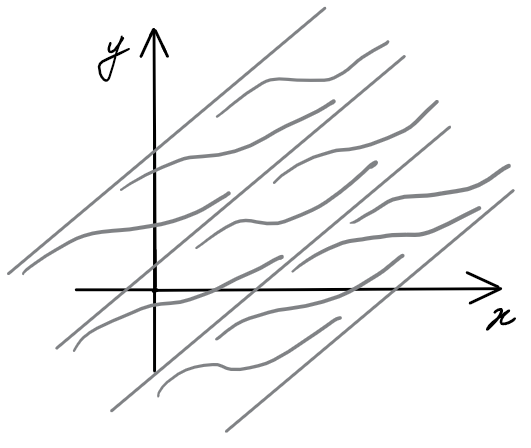
\includegraphics[width=55mm]{2_2_1.png}
            \caption{}
        }
    \end{figure}
\end{Example}